% !TeX spellcheck = en_US
\documentclass[a4paper]{scrartcl}

\usepackage[utf8]{inputenc}
\usepackage[english]{babel}
\usepackage[T1]{fontenc}
\usepackage{lmodern}
\usepackage{amsmath}
\usepackage{amssymb}
\usepackage{pdflscape}
\usepackage{geometry}
\usepackage{xcolor}
\usepackage{graphicx}
\usepackage{siunitx}
\usepackage{todonotes}
%\setlength{\parindent}{0pt}

\usepackage{biblatex}
\addbibresource{references.bib}


\geometry{a4paper, top=25mm, left=30mm, right=20mm, bottom=30mm,
headsep=10mm, footskip=12mm}

\newcommand{\itab}[1]{\hspace{0em}\rlap{#1}}
\newcommand{\tab}[1]{\hspace{.2\textwidth}\rlap{#1}}
\newcommand{\N}{\mathbb{N}}
\newcommand{\es}{\emptyset}

\title{Seminar on Algorithms for Compressed Graphs \\ Succinct Representation of Labeled Graphs}
\author{Matthias Dürksen}
\date{\today}
 

\begin{document}
\maketitle

\section{abstract}
Abstract erstellen
\begin{abstract}
	Inhalt...
\end{abstract}
Abstract (5 sentences)
+ What is the problem solved by the paper (or approach)? (1-2 sentences)
+ Why and for whom is the problem relevant? (1 sentence)
+ What is the essence of the solution to the problem? (1-2 sentences)
+ What is the benefit of the solution to the general public
or to other computer scientists or users? (1 sentence)


\section{Introduction}\label{sec:introduction}

1. Introduction
1.1. Motivation
- In which situations does the problem occur? Why and for whom is the solution important?
( 6 lines up to 1/3 page )
1.2. Which fundamentals are needed to understand t he paper – and where (i.e. in which text
books, papers, ...) to find them? (usually, a few sentences)
1.3. In which aspects does the paper that you present provide scientific contributions that go
beyond these fundamentals? (usually, a few sentences)

\subsection{Motivation}

\subsection{Fundamentals}

\subsection{Header}





\section{Main Part}
Ziel ist es eine Graphen möglichst effizent zu kodieren und dabei Query Anfragen effizent verarbeiten zu können. Dafür werden triangulierte planare Graphen in zu drei Bäumen umgewandelt, welchen wiederum in Klammerdarstellungen überführt werden. Die Klammerdarstellungen für die drei Bäume werden dann zu einer verschachtelten Klammerdarstellung umgewandelt. Diese Klammerdarstellung ist die effizente Kodierung, wo Anfragen effizient beantwortet werden können.




\subsection{Graph Model}
\todo{Änderung: Erst triangulated und anschließend als Erweiterung?}
Ein Graph $G=(V,E)$ besteht aus einener Menge von Knoten $V$ und einer Menge von Kanten $E$. Wir betrachten hierbei ungerichtete Graphen, sodass die Menge der Kanten $E$ ungerichtet ist.
Die Succint Representation  ist so aufgebaut, dass die Kodierung nur für eine Teilgruppe von Graphen, den ungerichteten planaren Graphen, funktioniert. Ein planarer Graph ist ein Graph $G$, welcher Knoten in einer zwei Dimensionalen Ebene dargestellt werden können, sodass sich keine Kanten mit einer anderen Kante schneidet. Ein Beispiel für einen planaren Graphen finden wir in Figure~\ref{fig:planar}.


\begin{figure}[h]
	\centering
	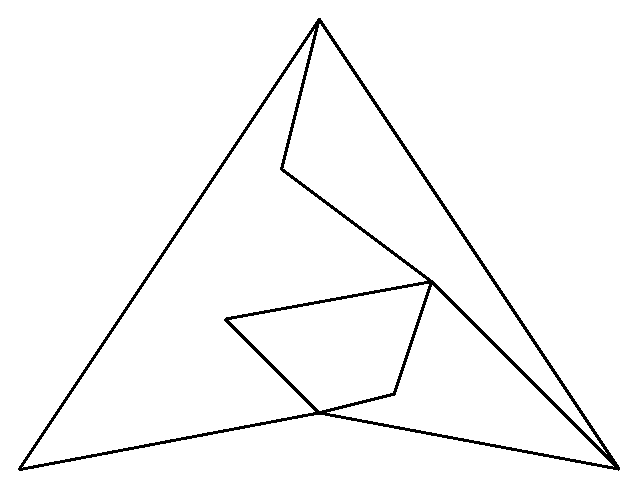
\includegraphics[width=0.7\textwidth]{img/planar}
	\caption{A planar graph}
	\label{fig:planar}
\end{figure}


Die planaren Graphen im ersten Schritt zu einen triangulierten planaren Graphen umgewandelt.
\todo{Explain how}
Der Graph aus Figure~\ref{fig:planar} wird durch den Graphen somit zu einem triangulated planar Graph, siehe Figure~\ref{fig:triangulated}.
\todo{Warum immer drei Eckpunkte}
Daher kann angenommen werden, dass der Graph immer drei Eckpunkte besitzt, welche jeweils adjazent zueinander sind. Diese Kanten bilden dabei die konvexe Hülle des Graphen, wobei wir die drei Knoten als $v_0,v_1$ und $v_{n-1}$ bezeichnen.


\begin{figure}[h]
	\centering
	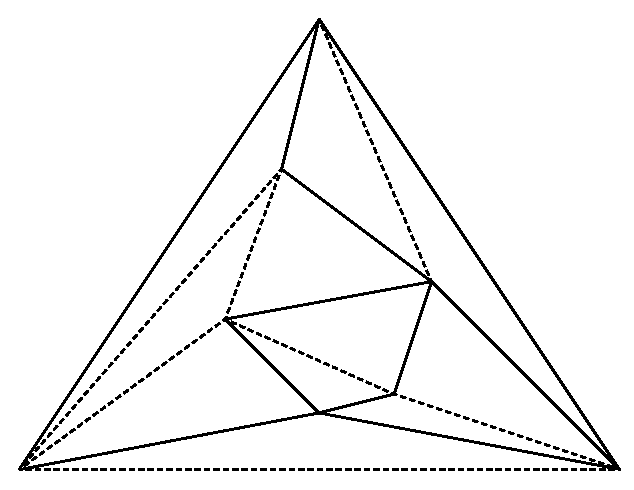
\includegraphics[width=0.7\textwidth]{img/triangulated}
	\caption{The triangulated  graph from Figure~\ref{fig:planar}}
	\label{fig:triangulated}
\end{figure}
\todo{Explain complexity for space/time}

\subsection{Schnyder Realizer}
Der Graph wird für die weitere Kompression in drei Bäume unterteilt. Dafür wir ein Schnyder Realizer~\cite{schnyder} benutzt. Dieser unterteilt den Graphen in drei Bäume $T_0,T_1,T_2$. Dabei wird jede innere Kante zu einem der drei Bäume zugeordnet. Diese werden so zugeordnet das jeder innere Knoten drei ausgehende Kanten hat, wobei jede ausgehende Kante einen anderen Baum enthalten ist. \todo{Explain: Why directed} Außerdem kann der Knoten noch eingehende Kanten haben, wobei diese bestimmt angeordnent sein müssen. In Figure~\ref{fig:schnyderRealizer} sehen wir die Anordnung. Dabei sind die Kanten nach dem Muster outgoing $T_0$, incoming $T_1$, outgoing $T_2$, incoming $T_0$, outgoing $T_1$, incoming $T_2$ angeordnent. Dabei haben die Bäume $T_0,T_1,T_2$ als Wurzel jeweils den Knoten  $v_0,v_1,v_{n-1}$.
Somit wird der Graph, siehe Figure~\ref{fig:example}, in drei Bäume unterteilt, siehe Figure~\ref{exampleSchnyder}.\todo{Vlt genauer erklären wie die Konstruktion zustande kommt}
\begin{figure}[h]
	\centering
	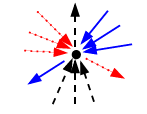
\includegraphics[width=0.7\textwidth]{img/schnyderRealizer}
	\caption{Structure of the edges for an internal node in the graph. }
	\label{fig:schnyderRealizer}
\end{figure}



\begin{figure}[h]
	\centering
	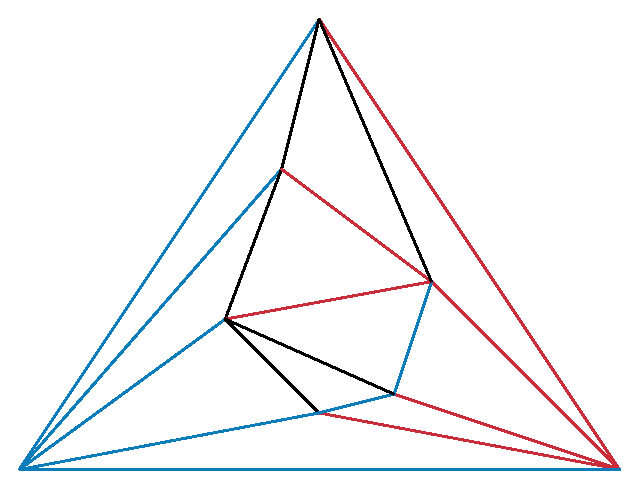
\includegraphics[width=0.7\textwidth]{img/exampleSchnyder}
	\caption{The trees in the graph which are formed on the basis of the Schnyder realizer}
	\label{fig:exampleSchnyder}
\end{figure}



\subsection{Traversal Orders}
Der Graph wird mittels  eines Schnyder Realizer zu drei Teilbäumen unterteilt, jedoch sind die Kanten, welche auf der Konvexen Hülle des Graphen liegen, noch nicht in den Bäumen enthalten. Außerdem müssen wir die Knoten für die anschließende Klammerdarstellung noch Nummerieren.\todo{warum werden die anderen Traversal Orders benötigt}
Die zwei Kanten $(v_1,v_0),(v_{n-1},v_0)$, welche auf der konvexen Hülle liegen, werden dabei dem Baum $T_0$ zugeordnet und die Kante $(v_{n-1},v_1)$ wird dem Baum $T_1$ zugeordnent. Somit ist $T_0$ an canonical spanning tree.

Um die Knoten zu Nummerieren wird in $T_0$ eine Tiefensuche im Knoten $v_0$ gegen den Uhrzeigersin ausgeführt und dabei die besuchen Knoten aufsteigend durchnummeriert, siehe Figure~\ref{fig:exampleTraversal}.

\begin{figure}[h]
	\centering
	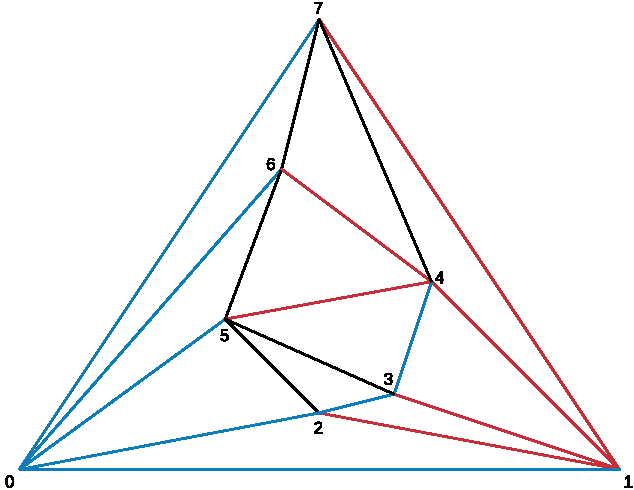
\includegraphics[width=0.7\textwidth]{img/exampleTraversal}
	\caption{The partitioned graph with the numbering by $T_0$}
	\label{fig:exampleTraversal}
\end{figure}




\subsection{Parenthesis}
Ziel ist es die Bäume mithilfe von Klammerdarstellungen zu einer gemeinsamen Klammerdarstellung zu kombinieren. Dafür generieren wir zunächst für die einzelnen Bäume die Klammerdarstellung und anschließend werden diese kombiniert. Für jeden der Bäume $T_0,T_1,T_2$ wird die Klammerdarstellung anders erzeugt. Dabei bezeichen wir ein Klammerpaar als eine öffnende Klammer welche von einer schließenden Klammer gefolgt ist.

Betrachten wir zunächst die Klammerdarstellung für den Baum $T_0$. Ausgehend von der Wurzel $v_0$ wird diese Klammerdarstellung erzeugt. Um die Wurzel zu kodieren nutzen wir Klammerpaar. Für jedes der Kinder der Tiefe 1 erstellen wir in dem Klammerpaar eine weitere Klammerpaar. Falls ein Kind $a$ der Tiefe 1 selber Kinder hat werden seine Kinder wiederum als Klammerpaar in dem Klammerpaar für den Knoten $a$ dargestellt. Dabei werden die Kinder auf einer Ebene entgegnen des Uhrzeigersinns in der Klammerdarstellung aufgenommen. Somit folgt folgende rekursive Definetion:

Für alle Knoten $v$ der Tiefe i gilt:



\begin{equation}
 &i=0 \rightarrow \text{pair of parenthesis}\\
 
&i>0 \rightarrow \text{insert pair of parenthesis in } parent(v)
\end{equation}
\todo{Geordnet}

Figure~\ref{fig:parenthesisTrees}a) zeigt wie eine solche Klammerdarstellung für den Baum $T_0$ anhand unseres Beispiel aussieht.

\begin{figure}[h]
	\centering
	\includegraphics[width=0.7\textwidth]{img/parenthesisTrees}
	\caption{The parentheses of the individual trees}
	\label{fig:parenthesisTrees}
\end{figure}




Für den Baum $T_1$ wird die Klammerdarstellung anderes generiert. Für jedes Kind der Wurzel $v_1$ wird ein Klammerpaar erstellt, jedoch werden die Klammerpaare nicht nacheinander auf die selbe Ebene geschrieben sondern inneinander geschachtelt. Hierbei werden die Kanten wieder gegen den Uhrzeigersinn durchgegangen, sodass das Kind $a$ , welches zuerst besucht wird, außen steht und die weiterne Kinder in das Klammerpaar von $a$ geschrieben werden. Falls ein Knoten $v$ Kinder hat werden die Kinder ebenfalls ineinander geschachtelt dargestellt und an die Stelle der Klammerungen gepackt, welche direkt nach der schließenden Klammer von $a$ kommt.\todo{example}. Die Klammerdarstellung für den Baum $T_1$ aus unserem Beispiel  wird in Figure~\ref{fig:parenthesisTrees}b) dargestellt.




Die Klammerdarstellung für den Baum $T_2$ wird ähnlich zu der Klammerdarstellung von $T_1$ erstellt. Erneut werden die Kinder wieder ineinander geschachtelt, jedoch werden die Kinder im Uhrzeigersinn durchgegangen. Wenn ein Knoten $v$ Kinder hat werden diese inneinander geschachtelten Kindern nun vor die öffnende Klammer von $v$ geschrieben. Dieses Verfahren wird anhand von dem Beispiel in Figure~\ref{fig:parenthesisTrees} deutlich.




Die drei Klammerdarstellungen  müssen nun so kombiniert werden, dass keine Information über den Graphen verloren geht. Die Klammerdarstellung eines Baumes $T_i$ bezeichen wir als $S_i$. Um die Teile der  unterschiedlichen Klammerdarstellungen nach der Kombination unterscheiden zu können, nutzen wir für Klammerdarstellungen jeweils andere Klammersymbole. Als Grundgerüst dient hierbei die Klammerdarstellung $S_0$. In diese werden die anderen beiden Klammerdarstellungen eingebunden. Die Klammerdarstellung wird wie folgt erstellt.

\begin{itemize}
	\item $\forall e=(v_i,v_j)\in T_1: \text{ insert } '[' \text{ before } parenthesis(v_i)\in S_0 \text{ closed.}$
	\item $\forall e=(v_i,v_j)\in T_1: \text{ insert } ']' \text{ after } parenthesis(v_i)\in S_0 \text{ opened.}$
	\item $\forall e=(v_i,v_j)\in T_2: \text{ insert } ']' \text{ after } parenthesis(v_i)\in S_0 \text{ opened.}$
	\item $\forall e=(v_i,v_j)\in T_2: \text{ insert } '[' \text{ before } parenthesis(v_i)\in S_0 \text{ closed.}$
\end{itemize}
In dem Beispiel werden die drei Klammerdarstellungen zu der kombinierten Darstellung in Figure~\ref{fig:parenthesisCombi}.
Darduch entsteht eine Klammerdarstellung die drei Typen von Klammern enthält, wobei jede Klammerdarstellung für sich immer noch eine gültige Klammerdarstellung ist.

\section{Size complexity}


Die Klammerdarstellung besteht aus drei verschieden Typen von Klammern, wobei für jeden Typen 2 Symbole benötigt werden (Öffnende und Schließende Klammer). Somit werden insgesamt 6 verschiedene Zeichen benötigt. Jede Kante des Graphen wird genau ein mal kodiert und pro Kante werden eine öffnende und eine schließende Klammer benötigt. Knoten müssen nicht extra mitkodiert werden, da die Informationen indirekt  die Kanten enthalten. Somit werden für die Darstellung $2m$ Symbole benötigt, bei m ist die Anzahle der Kanten in G.



\section{Reconstruction of the graph}


\section{Conclusion \& Future Work}
3. Conclusions (0,5 pages)
3.1. Greatest highlights of the paper
3.2. Benefit of the suggested solution



\section{Literature}

4. Complete literature references (cited completely and correctly)
For Journals:
<Authors> : <Title> . <italics:Journal> , <italics:Volume> , <Number>, <Year> , <Pages> .
Example:
A. Lempel and J. Ziv: A universal algorithm for sequential data compression. IEEE Transactions
on Information Theory, 23(3) 1977, pp. 337–343.
For conference papers and workshop papers:
<Authors> : <Title> . <Conference title> , <Conference city> , <Conference country>, <Month> ,
<Year> .
Example:
S. Mantaci, A. Restivo, G. Rosone, and M. Sciortino: An extension of the Burrows Wheeler
transform and applications to sequence comparison and data compression, in Combinatorial
Pattern Matching, CPM 2005, Proceedings, vol. 3537 of LNCS, Springer, 2005, pp. 178–189.



\pagebreak

\nocite{*}
\printbibliography







\end{document}